\newcommand{\E}{\mathbb{E}}

Constructing a strict rate-limiting protocol for multi-party communication requires complete knowledge of all the senders in the system and their sending rates. However this is difficult to achieve without using a centralized server or running a consensus protocol. This is specially the case for systems comprised of multiple non-overlapping groups where nodes do not receive all the multicast messages pushed on the network.

We note that a minor relaxation of the requirements can result in a simple decentralized solution to the rate-limiting problem. Rather than enforcing a strict or `hard' aggregate limit at all times, we will allow occasional and temporary violations, i.e. a `soft' limit. Thus, our goal will be to minimize the frequency of the global limit violations.

An optimal dynamic multi-party rate-limiting protocol uses global information regarding the aggregate traffic rate, and the rates on different channels, and makes decisions to dynamically slow down certain nodes or adjust the bandwidth quota allotted to certain groups. However, The relaxed requirement allows us to build \sysname{} in a decentralized fashion such that nodes can use local information to estimate the global traffic rates and make decisions on which nodes should slow down, and how should the bandwidth quotas be readjusted.

On a high level, a node running the \sysname{} protocol will send multicast messages without restrictions and periodically reevaluate its sending bandwidth quota as to not exceed the global limit. When the limit is exceeded, nodes will apply an administrator-specified \textit{slowdown} policy to reduce their sending rate.

\sysname{} runs in equal-sized time windows, or \textit{epochs}, and has two parts:
\begin{itemize}
\item A \emph{monitor} gathers statistics about multicast use on the network.

\item A \emph{reactor} is activated at the end of each epoch if traffic rates reach a critical threshold of the limit $L$. The reactor reevaluates sending quotas and invokes slowdown policies.
\end{itemize}

Nodes use local estimates obtained by the monitor to evaluate whether the global limit has been exceeded. When the limit is exceeded, a subset of the nodes and groups are designated as a \textit{Reaction Domain} and are required to slow down their sending rates and cut their bandwidth quotas.

\subsection{The Monitor}
Monitors are used to collect local information that estimate the global status of the system. \sysname{} implements the monitor component using a global dedicated broadcast channel. At the end of each epoch, nodes probabilistically broadcast the total amount of traffic that has been sent in the groups they belong to in the previous epoch. This allows all monitoring nodes to track the total multicast use in a decentralized fashion without promiscuously listening for traffic in other groups.

Upon receiving an update $r_j$, the monitor will store it until another update about $G_j$ is received, or for a finite timeout period after which the transmission rate on $G_j$ is assumed to be 0.

The broadcast probability determines the expected accuracy of the local information at each node. The network administrator specifies the expected amount of broadcast traffic to be used for the monitor as a fraction ($c$) of the total amount of multicast used by the rest of the system. At the end of each epoch $t$, a node $n_i \in G_j$ sends a broadcast message with probability $c \cdot \dfrac{r_j(t)}{|G_j|}$.

\begin{claim}
The expected rate of reports published on the broadcast channel is a $c$ fraction of the total multicast traffic in the system.
\end{claim}

\begin{proof}
Assume the multicast traffic rate for group $G_j$ is a constant $r_j = r_j(t)$ for all $t$.
For a fixed a group $G_j$ let
\[
t_{ij} = \left\lbrace \begin{array}{ll} 1 & \textrm{ if node $i$ in $G_j$ sends a report packet} \\
0 & \textrm{ otherwise} \end{array} \right.
\]

Let $t_j = \sum_{i=1}^n t_{ij}$ denote the rate of packets sent to the broadcast channel that deal with group $G_j$. The total rate of packets sent to the broadcast channel is $T = \sum_{j=1}^m t_j$. We have
\begin{eqnarray*}
\E[T] &=& \sum_{j=1}^m \sum_{i=1}^n \E[t_{ij}] \\
&=& \sum_{j=1}^m \sum_{i \in G_j} c \frac{r_j}{|G_j|}  \\
&=& c \sum_{j=1}^m r_j,
\end{eqnarray*}
by the linearity of expectation, which proves the claim.
\end{proof}


\subsubsection{Smoothed Rate Aggregation}
To filter out the effects of spikey sending rates, monitors can keep track of an exponential moving average (EMA) of the communication rates of other nodes and groups. More specifically, let $0 < \gamma \leq 1$ be the \textit{smoothing factor} for the exponential moving average function. Each node records
\[ r_j(t) = \gamma \cdot o_j(t) + (1 - \gamma) \cdot r_j(t-1) \]

where $o_j(t)$ is the observed communication rate of $G_j$ during epoch $t$. Notice that by setting $\gamma = 1$ we will have $r_j(t) = o_j(t)$.


\subsection{The Reactor}
Nodes activate their reactor component when aggregate traffic rates reach a critical threshold of the limit $L$. Each node uses its local estimates to independently compute whether it is part of the reaction domain or not. Nodes in the reaction domain will apply a slowdown policy adjusting the bandwidth quotas for subsequent epochs.

\subsubsection*{Reaction Domains}
A reaction domain is defined as the top $\beta$ highest traffic nodes in the top $\alpha$ highest traffic groups. For this we explicitly define $0 < \alpha \leq 1$ to be the fraction of the highest traffic groups to be included in the domain, and $0 < \beta \leq 1$ to be the fraction of the highest traffic nodes to be included in the domain.

At the end of epoch $t$, node $n_i$ in group $G_j$ uses the information supplied by the monitor to compute the reaction domain. $n_i$ determines if $G_j$ is in the reaction domain by computing if:

\begin{center}
\verb|rank of| $G_j$ \verb|by traffic| $\leq \lceil \alpha M \rceil$\\
(i.e. if $G_j$ is one of the top $\alpha$ groups)
\end{center}

If so, $n_i$ checks if:
\begin{center}
\verb|rank of| $n_i$ \verb|by traffic in| $G_j \leq \lceil \beta |G_j| \rceil$\\
(i.e. if $n_j$ is one of the top $\beta$ senders in group $G_j$)
\end{center}

If so, $n_i$ is in the reaction domain and applies the slowdown policy in subsequent epochs.

\begin{figure}[t]
 \centering
 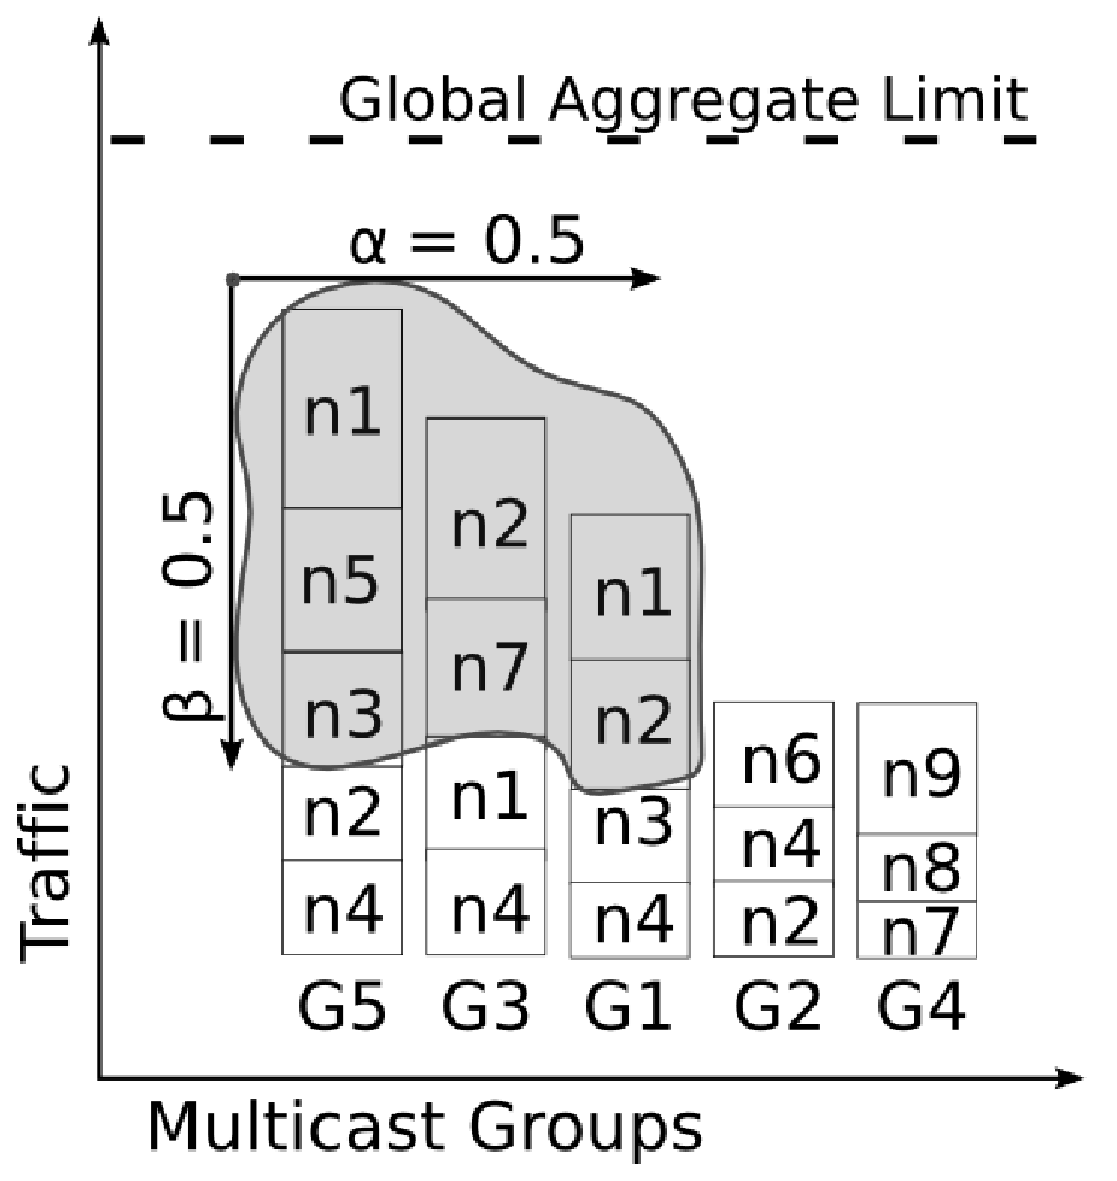
\includegraphics[scale=0.4]{figures/reaction-domain-bubble-gray.eps}
 \caption{An illustration of a reaction domain configured with parameters $\alpha=0.5, \beta=0.5$. The reaction domain (shaded area) encompasses the top $\beta$ senders in the top sending $\alpha$ groups.}
 \label{ill:reaction-domain}
\end{figure}

Figure ~\ref{ill:reaction-domain} shows an illustration of a reaction domain computed in an instance with five sending groups. The groups are sorted decreasingly by traffic from left to right, and the senders within each group are sorted decreasingly by traffic in that group from top to bottom. The reaction domain then is computed by taking the top $\beta$ senders in the first $\alpha$ groups. Notice that this construction means that the reaction domain can change in different epochs. Additionally, the use of local estimates implies that different nodes might have different estimates for the reaction domain in this epoch. 
